\section{Optimization}
\label{sec:optimization}
In this section, we describe several optimizations to the star-partition and mining algorithm.
In addition, we also address some practical issues when deploying the SPM algorithm
to real MapReduce based systems.

%We have analyzed that the bottlenecks of Algorithm~\ref{algo:apriori_mining} 
%lies in two factors. The size of each $Sr_s$ and the size of candidates in each level of Apriori.
%In this section, we provide several optimizations to boost the bottlenecks.
%\subsection{Edge Reduction by Direction}
%The first spot for reducing the size of $Sr_s$ is to remove the replicated edges. As shown in Algorithm~\ref{algo:spm_overview}, each edge in the conceptual graph is replicated twice in generating the star-structure. The purpose of replication is to ensure the completeness of star partition. However, this replication can be avoided if we choose an appropriate way of partitioning. 
%
%We design the edge partitioning method by edge direction. Instead of building a conceptual graph that is undirected, we create the directed conceptual graph as follows: First, we assign each object a unique number. Then
%for a cluster $C_t$ in snapshot $S_t$, for any pair $(u,v) \in C_t$, an edge $e(u,v) = \{t\}$ is created if $u < v$. It is easy to see that the directed conceptual graph is a DAG. We then create each $Sr_u$ by including all the outgoing edges of $u$. By so doing, each edge is assigned to only one star, thus avoids the replications. We use the following theorem to ensure the completeness of the edge direction method.
%
%\begin{theorem}[Sound and Completeness of Edge Direction]
%Star partition with edge direction is sound and complete.
%\end{theorem}
%\begin{proof}
%It is notable that each star is a subset of original trajectories, thus the soundness is trivially true. For completeness, if $P$ is valid pattern, then let $s$ be the object of the smallest number in $P.O$, i.e., $s=\min_{o \in P.O}(o)$. Since $s$ is smallest and the all other objects in $P.O$ is connected with $s$. Therefore, $P.O \equiv Sr_s$, which indicates that $P.O$ is also a pattern in $Sr_s$.
%\end{proof}
%An example of edge direction is shown in Figure~\ref{fig:star_partition}. As shown,
%by adapting the direction method, half the size of $S_r$'s is reduced. This clearly brings efficiency in both shuffling and apriori mining.

\subsection{Edge Simplification}
Each edge $e(s,v)$ in $Sr_s$ contains a time sequence $ET$ 
which represents the co-occurrence of $s$ and $v$. We notice that the edge 
between $s$ and $t$ is not always necessary. For example, if an edge has a
cardinality less than $K$, it is unnecessary to include this edge to 
$Sr_s$ since it cannot contribute to any patterns.
This motivates us to simplify the edges in $Sr_s$ 
to boost the overall performance.

Our goal of edge simplification is to, given a time sequence $T$, find a subsequence
of $T' \subseteq T$, such that $T'$ is potentially conforms to $K,L,G$. And we
wish $|T'|$ to be as small as possible.  
We star-off by observing that for every time sequence $T$, $T$ can be 
divided into a set of maximally $G$-connected subsequences. Note that
a maximally $G$-connected subsequence can potentially contribute to
a pattern if it conforms to $K,L$.
Therefore, we are able to reduce $T$
to its maximally $G$-connected subseuqnces which conform to $K,L$.

To formally describe the idea, we define the \emph{candidate sequence} as follows:

%\begin{definition}[Candidate Sequence]
%Given the pattern parameters: $K,L,G$, a sequence $T$ is 
%a \emph{partly candidate} sequence if exists one of its maximal $G$-connected
%subsequence $T'$ such that $T'$ confirms to $L,K$.
%\end{definition}

%For example, let $L = 2, K = 4, G = 2$, sequence $T_1=(1,2,4,5,6,9,10,11)$ 
%is a \emph{partly candidate sequence} since $T_1[1:5] = (1,2,4,5,6)$ is a valid
%pattern wrt. $L,K,G$. In contrast, $T_2=(1,2,5,6,7)$ is not a valid partly candidate sequence.
%
%Observing that only partly candidate sequence can be potentially contribute to a 
%pattern. Therefore, given an edge $e(s,t)=T \in Sr_s$, if $T$ is not a partly
%candidate sequence, it can be pruned from $Sr_s$. To efficiently
%test whether a given sequence is partly candidate, we define the \emph{Fully Candidate Sequence}:

\begin{definition}[Candidate Sequence]
Given the pattern parameters: $L,K,G$, a sequence $T$ is a \emph{Candidate Sequence} 
if for any of its maximal $G$-connected sequence $T'$, $T'$ conforms to $L,K$.
\end{definition}

For example, let $L = 2, K = 4, G = 2$, sequence $T_1=(1,2,4,5,6,9,10,11,13)$ is 
not a fully candidate sequence since one of its maximal $G$-connected sequence $(9,10,11)$
is not a partly candidate sequence. In contrast, sequence $T_2=(1,2,4,5,6)$ is 
a fully candidate sequence.

To reduce a sequence $T$ to a candidate sequence, we need to strip out its 
maximal $G$-connected subsequences which does not form to $K,L$. Such a reduction
takes two rounds scan of $T$ as shown in Algorithm~\ref{algo:simp_prune}. In the 
first round, the consecutive portions of $T$ with size less than $L$ are removed.
In the second round, the maximal $G$-connected sequences of size less than $K$ are
removed. Clearly the simplification algorithm runs in linear time.
\begin{algorithm}
\caption{Edge Simplification}
\label{algo:simp_prune}
\begin{algorithmic}[1]
\Require $T$
\State{---Remove the consecutive segment with size less than $L$---}
\State $c \gets 0$
\For {$i \in (0,...,|T|)$}
	\If{$T[i] - T[i-1] != 1$} 
		\If{$i - c < L$} 
			\State $T$ remove $[c:i)$
		\EndIf
		\State $c \gets i$
	\EndIf
\EndFor
\State{---Remove the $G$-connected segment with size less than $K$---}
\State $s\gets 1$, $c\gets 0$
\For{$i \in (0: |T|)$}
	\If{$T[i] - T[i-1] > G$}
		\If{$s < K$}   
			\State $T$ remove $[c:i)$
		\EndIf
		\State {$c \gets i$, $s \gets 1$}
	\Else
		\State $s++$
	\EndIf
\EndFor
\end{algorithmic}
\end{algorithm}

\begin{example}
Take $T_1=\{1,2,4,5,6,9,10,11,13\}$ as an example of edge simplification. Let $L = 2, K = 4, G = 2$.
In the first round of scan. $T_1$ reduces to $\{1,2,4,5,6,9,10,11\}$. The consecutive subsequence $\{13\}$
is removed by $L=2$. $T_1$ has two maximal $G$-consecutive subsequences, which 
are $\{1,2,4,5,6\}$ and $\{9,10,11\}$. Since $K=4$, $\{9,10,11\}$ is removed
from $T_1$ in the second round of scan. Therefore, $T_1$ is simplified to $\{1,2,4,5,6\}$.
\end{example}

%
%Based on the fully candidate sequence, we can reduce an sequence $T$ to a 
%fully candidate sequence by striping out its non-partly candidate maximal pseudo-consecutive 
%sequences. The reduction works as in Algorithm~\ref{algo:simp_prune}. It takes two
%rounds of scan of an input $T$. In the first round of scan,
%the consecutive portion of $T$ with size less than $L$ is removed.
%In the second round of scan, the pseudo-consecutive portion of $T$ with size less than $K$
%is removed. 


By leveraging the edge simplification technique, 
the size of the edges in $Sr_s$ can be greatly reduced. If
an edge cannot be reduced to a candidate sequence, then it is directly removed from $Sr_s$.
If an edge can be reduced to a candidate sequence, replacing itself 
by the candidate sequence results in a more compact storage.

%We use the following theorem to state the completeness and correctness of the 
%edge reduction algorithm.
%\begin{theorem}[Soundness and Completeness Edge Simplification]
%Star partition with edge simplification is sound and complete.
%\end{theorem}
%
%\begin{proof}
%Soundness of the star partition is not affected by edge simplification since each star is a subset of original trajectory. For completeness, notice that given a time sequence $T$, and any of its maximal $G$-connected subsequence $T'$, if $T'$ does not conform to $L,K$, then $T'$ cannot contribute to any patterns. 
%\end{proof}


\subsection{Candidate Pruning}
\subsubsection{Temporal monotonicity}
During the apriori phase, we repeatedly join candidate patterns in different levels to generate a larger set
of a patterns. We observe that traditional monotonic property of Apriori algorithms \textbf{does not}
hold in GCMP mining. That is given two candidate $P_1, P_2$, if $P_1.O \subset P_2.O$ and $P_1$ is not 
a valid pattern, then $P_2$ may or may not be a valid pattern. However, we notice that
we may form another monotonic property based on the \emph{candidate sequence} such that
the Apriori algorithm could still benefit.

The intuition is that if a candidate $P_1.T$ cannot be reduce to a \emph{candidate sequence}, then $P_1$ cannot 
be valid pattern. Furthermore, any candidate $P_2$, with $P_1.O \subset P_2.O$ cannot be a valid pattern.
This \emph{temporal monotonic property} 
is explicitly described as in the follow theorem:

\begin{theorem}[Temporal Monotonic Property of GCMP]
Given the temporal parameters $L,G,K$, for a candidate $c$ in Algorithm~\ref{algo:apriori_mining},
if $c.T$ cannot be reduced to a candidate sequence, then for any candidate $c'$ with $c.O \subset c'.O$, $c'$ can be pruned.
\end{theorem}
\begin{proof}
Let $c_1$, $c_2$ be two candidates with $c_1.O \subset c_2.O$. It is easy to see that $c_1.T \supseteq c_2.T$.
If $c_1.T$ cannot be reduced to a candidate sequence, then any subset of $c_1.T$ cannot
be reduced. It follows that $c_2.T$ cannot be reduced neither. Thus,
if $c_1.T$ cannot be reduced to a candidate sequence, $c_2$ can be pruned. 
\end{proof}

\subsubsection{Forward closure checking}
Although leveraging \emph{temporal monotonicity} could largely prune false candidates and reduce
the apriori search space, it is ineffective when a \textit{true} pattern exists. 
For example, if a final pattern of a star $Sr_s$ is the \textit{union of all vertices} in the star, 
then in apriori, ${|Sr_s|}\choose{i + 1}$ candidates needs to be generated at 
each level $i$. This results in an exponential search space while
the output only contains one pattern.  
In general, when candidates at level $i$ collectively forms a true pattern, 
running aprior produces many wasted candidates. 

Let $Lv_i$ be the set of candidates at level $i$ of Algorithm~\ref{algo:apriori_mining},
we use the \emph{forward closure} $FC_i$ to denote the union of the objects in
all candidates in $Lv_i$. Then, the \emph{forward closure checking} is stated as follows:
\begin{theorem}[Forward Closure Checking Rule]
Let $Lv_i$ be the candidates generated at level $i$ in Algorithm~\ref{algo:apriori_mining},
if $FC_i$ is a proper pattern, then it is safe to terminate Algorithm~\ref{algo:apriori_mining}
and directly output $FC_i$.
\end{theorem}

\begin{proof}
We prove by contradiction. Suppose there exists another pattern $P$ such that $P.O \neq FC_i$, let 
$X=P.O - FC_i \neq \emptyset$. Consider a subset of $P$ which contains $X$ with size $i+1$, (i.e., $P_1 \subseteq P, P_1\subseteq X, |P_1|=i+1$). Since $P$ is a proper pattern, then $P_1$ is also a proper pattern. Therefore $P_1 \in Lv_i$.
Then it follows $X$ is in the forward closure of $FC_i$, (i.e.,$X \in FC_i$), which contradicts with $X\notin FC_i$.
\end{proof}

It is notable that, as the level grows in Algorithm~\ref{algo:apriori_mining}, the closure $FC$
reduces, thus the pruning power of $FC$ would be stronger.

%To facilitate efficient mining, we adapt the \emph{forward closure checking} rule to 
%quickly determine whether it is sufficient to terminate the apriori search. Given the candidates at
%level $i$ $Lv_i$, we define the \emph{forward closure} of $Lv_i$ as the union of objects from
%all candidates. Then, the following \emph{forward closure checking} rule can be used:
%
%\begin{theorem}[Forward Closure Checking Rule]
%Let $Lv_i$ be the candidates generated at level $i$ in Algorithm~\ref{algo:apriori_mining}, the forward closure
%is $\mathbb{F}_i = \cup_{cand \in Lv_i} (cand.O) $. Algorithm~\ref{algo:apriori_mining} terminates when 
%$FC_i$ forms a valid GCMP .
%\end{theorem}

\begin{example}
We use Figure~\ref{fig:star_partition} (c) to 
demonstrate the power of candidate pruning. 
As shown, at the initial stage, $\{3,6:3\}$ is first pruned by \textit{Edge Simplification} since its
timestamps fails to be a candidate sequence. Subsequently, all further candidates containing $\{3,6\}$ 
are pruned by \textit{Temporal Monotonicity}. Then, we check the \textit{Forward Closure} 
of remaining candidates (i.e., $\{3,4\}$ and $\{3,5\}$) and find $\{3,4,5\}$ is a
valid candidate. Therefore, $\{3,4\}$ and $\{3,5\}$ are pruned, and $\{3,4,5\}$ is the output.
\end{example}
%
%With the help of the \emph{Monotonic Property}, the number of new candidates in each level is greatly reduced. We verify this in the experiment session as well.

\subsection{Star Partition Analysis}
As we see in Section~\ref{sec:spm_solution}, the apriori phase in SPM may
take exponential time. An important factor affecting the performance of
SPM is the size of stars. We notice that, the
size of star is related to the way the vertexes are numbered. 

\begin{figure}[h]
\centering
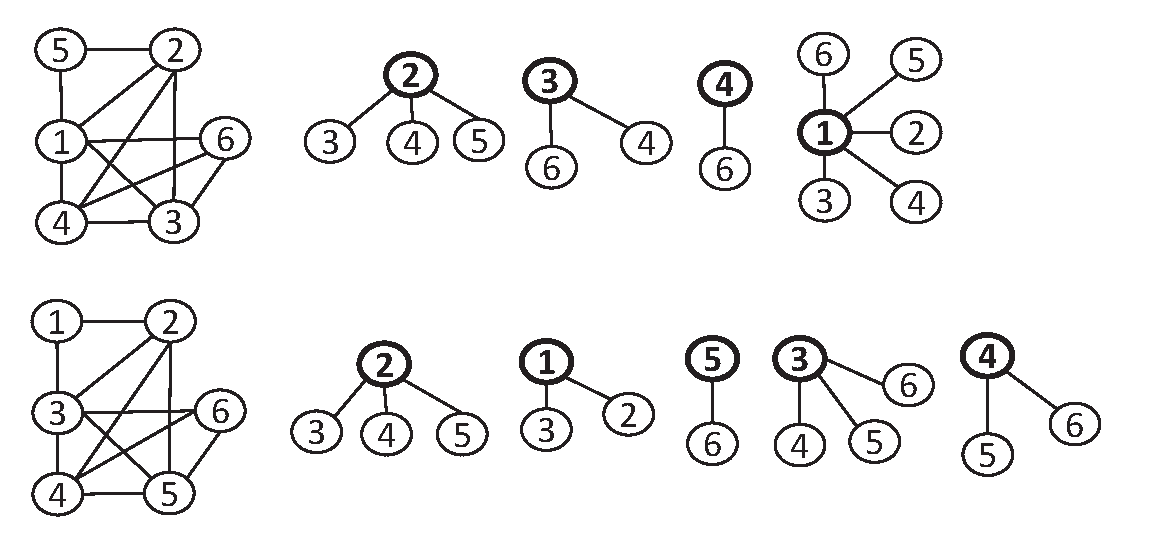
\includegraphics[width=0.4\textwidth]{star-alt.eps}
\caption{An alternative numbering and partitioning of the connection graph in Figure~\ref{fig:star_partition}.}
\label{fig:star-alt}
\end{figure}

For example,
Figure~\ref{fig:star-alt} gives an alternative numbering of vertexes 
in connection graph thus produces a different set of stars. This partitioning constructs
four stars with the maximum star consisting of 5 edges. Compared to the partitioning
in Figure~\ref{fig:star_partition}(b) where five stars are produced with maximum star of 3 edges, this
partition is inferior in two aspects. First, this partition lacks of one star, which
results in a smaller number of parallelism. Second, this partition has a larger size
of maximum edges. With the exponential time complexity in Apriori, the largest star takes
much more time to compute.

The example shows that different numbering of vertexes in connection graph indeed affects
the SPM performance. Therefore we wish to find a numbering scheme of connection graph
such that the edges in each star are best distributed. Notice that the sum of edges 
is invariant for any numbering scheme of the graph. Thus, our goal is equivalent to find
a numbering such that the maximum edge size from all stars is minimized. 

To formalize the objective, we design an linear algebra model as follows: Let $G$ denote a connection graph.
Let $\mathbb{A}$ be an arbitrary numbering of vertexes in $G$.
Let $(A:a_{i,j})$ be the matrix representing the induced graph wrt. $\mathbb{A}$. Let vector $\vec{b}$
be the \textit{one}\footnote{Every element in $\vec{b}$ is $1$} vector. Let $\vec{c}:c_j$ be the
vector equals to $A\vec{b}$. It is easy to see that each $c_j$ denotes the size of star for vertex $j$.
Therefore, the objective of load balancing can be formalized as follows:
\begin{equation}
\mathbb{A}  = \argmin(||A\vec{b}||_\infty) \text{,where } ||A\vec{b}||_\infty = \max_{1\leq j \leq n}(c_j)
\end{equation}

Though the objective is well-defined as above, it is challenging to directly optimize
the equation. First, suppose there are $n$ vertex in $G$, enumerating
all possible $\mathbb{A}$s leads to $n!$ combinations. 
Such a high complexity is trivially unpractical. Second,
since $G$ is constructed at runtime, 
the load planning can only start after $G$ is created. 
The planning time are thus required to be short enough otherwise the benefit cannot payoff the planning time.

Despite these challenges, we observe that there is a 
$O(1)$ time solution which is good enough as stated in the 
following theorem.

\begin{theorem}[Balance of Star Partition]
Let $G$ be a connection graph with $n$ vertexes and the average degree $d$.
Let $\mathbb{A}^*$ be the optimal numbering wrt. Equation 1.
For any numbering, $\mathbb{A}$, with high probability, the 
absolute difference between $\mathbb{A}^*$ and $\mathbb{A}$ is $O(\sqrt{n \log n})$.
That is, it is very likely that 
$||\mathbb{A}\vec{b}||_\infty = ||\mathbb{A}^*\vec{b}||_\infty + O(\sqrt{n \log n})$.
\end{theorem}

\begin{proof}
Let $\mathbb{A}^*$ be the optimal solution wrt Equation 1. Since we have a star
for each object, by the degree-sum formula and pigeon-hole theorem, $||A^*\vec{b}||_\infty \geq d/2$.
Next, let $e_{i,j}$ be a 0-1 indicator variable determining whether vertex $i$ connects vertex $j$
in $G$. Note that edges in $G$ are independent. We use $d_i$ 
to denote the degree of object $i$ in $G$.  It follows that $E[d_i]=E[\Sigma_{1\leq j \leq n}e_{i,j}]=d$.
Since in the star partition, each edge is assigned to the ending vertex
with lower ID, the connection between $a_{i,j}$ and $e_{i,j}$ can be written as:
\begin{equation*}
a_{i,j} = \begin{cases}
			e_{i,j}, i>j \\
			0, otherwise
		  \end{cases}  
\end{equation*}
There are two observations made on the above equation. First, since $e_{i,j}$s are independent,
$a_{i,j}$s are independent. Second, since $i>j$ and $e_{i,j}$ are independent. 
$E[a_{i,j}] = E[e_{i,j}]E[i>j]= E[e_{i,j}]/2$.

By definition, $c_i = \Sigma_{1\leq j \leq n} a_{i,j}$, 
is a sum of $n$ independent 0-1 variables. Taking expectation on both sides, 
we get: $E[c_i] = E[\Sigma_{1\leq j \leq n} a_{i,j}]=E[\Sigma_{1\leq j \leq n} e_{i,j}]/2 = d/2$. Let $\mu =E[c_i] = d/2$, 
$t = \sqrt{n\log n}$, by Hoeffding's Inequality, the following holds:
\begin{equation*}
\begin{split}
	Pr(c_i \geq \mu + t) 
						&\leq \exp(\frac{-2t^2}{n}) \\
						&= \exp(-2\log n) = n^{-2}
\end{split}
\end{equation*}

The first step is due to the fact that all $a_{i,j}$ are bounded in the range of [0,1]. 
Next, since the event $(\max_{1\leq j \leq n}(c_j) \geq \mu + t)$ can be viewed as
$\cup_{c_i} (c_i \geq \mu + t )$, by Union Bound, we achieve the following:
\begin{equation*}
\begin{split}
	Pr(||A\vec{b}||_\infty \geq \mu + t) &=Pr(\max_{1\leq j \leq n}(c_j) \geq \mu + t)  \\
		& = Pr(\cup_{c_i} (c_i \geq \mu + t )) \\
		&\leq \Sigma_{1 \leq i \leq n} Pr(c_i \geq \mu + t) \\
		& = n^{-1} = 1/n
\end{split}
\end{equation*}
Substitute $t$ and $\mu$, we achieve the following concise form:
\begin{equation*}
	Pr(||A\vec{b}||_\infty \geq (d/2 + \sqrt{n\log n})) \leq 1/n
\end{equation*}
This indicates that, the probability of $(||A\vec{b}||_\infty-d/2)$ being less than or equal to $ O(\sqrt{n\log n})$ is $(1-1/n)$. With the observed fact that $||A^*\vec{b}||_\infty \geq d/2$, we conclude that
with probability greater than $(1-1/n)$, 
the difference between $||A\vec{b}||_\infty$ and $||A^*\vec{b}||_\infty$ is less than $O(\sqrt{n\log n})$.
\end{proof}

In fact, we have a tighter bound of $||A\vec{b}||_\infty -||A^*\vec{b}||_\infty$ if 
the connection graph is \emph{dense}. Specifically, if $d\geq \sqrt{12\log n}$, the following
equation holds:
\begin{equation*}
Pr(||A\vec{b}||_\infty \geq (d/2 + O(\sqrt{d\log n})) \leq 1/n
\end{equation*}

Induced by the Theorem 5, taking object IDs as the numbering (i.e., in Algorithm~\ref{algo:spm_overview})
would be guaranteed to produce a partition which is almost optimal.
%By definition, $c_i = \Sigma_{1\leq j \leq n} a_{i,j}$, is a sum of $n$ independent 0-1 variables.
%Taking expectation on both sides, we get: $E[c_i] = E[\Sigma_{1\leq j \leq n} a_{i,j}]=E[\Sigma_{1\leq j \leq n} e_{i,j}]/2 = d/2$. Let $\mu =E[c_i] = d/2$, $\delta = \sqrt{12\log n/d}$, by Chernoff Bound, 
%the following holds:
%\begin{equation*}
%\begin{split}
%	Pr(c_i \geq (1+ \delta)\mu) & \leq \exp(-\mu \delta^2 / 3) \\
%						&= \exp(-d/2 \times 12 \log n / 3d ) \\
%						&= \exp(-2\log n) = n^{-2}
%\end{split}
%\end{equation*}
%
%Next, since the event $\max_{1\leq j \leq n}(c_j) > (1+ \delta)\mu$ can be viewed as
%$\cup_{c_i} (c_i > (1+ \delta)\mu )$, by Union Bound, we achieve the following:
%\begin{equation*}
%\begin{split}
%	Pr(||A\vec{b}||_\infty > (1+ \delta)\mu)) &=Pr(\max_{1\leq j \leq n}(c_j) > (1+ \delta)\mu)  \\
%		&\leq \Sigma_{1 \leq i \leq n} Pr(c_i \geq (1+ \delta)\mu) \\
%		& = n^{-1} = 1/n
%\end{split}
%\end{equation*}
%Substitute $\mu$ and $\delta$, we achieve the following concise form:
%\begin{equation*}
%	Pr(||A\vec{b}||_\infty > (d/2 + \sqrt{3 d\log n})) \leq 1/n
%\end{equation*}
%This indicates that, the probability of $(||A\vec{b}||_\infty-d/2)$ being less than $ O(\sqrt{d\log n})$ is $(1-1/n)$. Notice that $||A^*\vec{b}||_\infty \geq d/2$, therefore, with probability greater than $(1-1/n)$, the difference between $||A\vec{b}||_\infty$ and $||A^*\vec{b}||_\infty$ is less than $O(\sqrt{d\log n})$.
%\end{proof} 
%
%Theorem 5 is powerful enough to induce the following lemma:
%\begin{theorem}[Load Balance of Algorithm~\ref{algo:spm_overview}]
%The partitioning in Algorithm~\ref{algo:spm_overview} differs at most $O(\sqrt{d\log |\mathbb{O}|})$ 
%from optimal partitioning with probability $(1-1/|\mathbb{O}|)$.
%\end{theorem}

